\documentclass[10pt,conference,final,letterpaper,twoside,twocolumn,]{IEEEtran}

\usepackage{graphicx}
\usepackage{color}
\usepackage{url}
\usepackage{ifpdf}
\usepackage{hyperref}
\usepackage{xspace}

\setlength\parskip{-0.015em}
\setlength\parsep{-0.15em}

\newenvironment{shortlist}{
	\vspace*{-0.85em}
  \begin{itemize}
 \setlength{\itemsep}{-0.3em}
}{
  \end{itemize}
	\vspace*{-0.6em}
}

\usepackage{fancyhdr}
\setlength{\headheight}{16.0pt}
\pagestyle{fancy}
\headheight = 0pt
\headsep    = 25pt
\fancyhf{}
\fancyhead[OC]{\bf {\it \footnotesize{Jha et al: A Case for SAGA as an Access Layer for DCI}}}

\newif\ifdraft
\drafttrue
\ifdraft
 \newcommand{\amnote}[1]{  {\textcolor{magenta} {***AM: #1}}}
 \newcommand{\jhanote}[1]{ {\textcolor{red}     {***SJ: #1}}}
 \newcommand{\tmnote}[1]{  {\textcolor{blue}    {***TM: #1}}}
\else
 \newcommand{\amnote}[1]{}
 \newcommand{\jhanote}[1]{}
 \newcommand{\tmnote}[1]{}
\fi

\newcommand{\dn}{\vspace*{0.33em}}
\newcommand{\dnn}{\vspace*{0.66em}}
\newcommand{\dnnn}{\vspace*{1em}}
\newcommand{\uppp}{\vspace*{-1em}}
\newcommand{\upp}{\vspace*{-0.66em}}
\newcommand{\up}{\vspace*{-0.33em}}
\newcommand{\shift}{\hspace*{1.00em}}

\newcommand{\T}[1]{\texttt{#1}}
\newcommand{\I}[1]{\textit{#1}}
\newcommand{\B}[1]{\textbf{#1}}
\newcommand{\BI}[1]{\B{\I{#1}}}
\newcommand{\F}[1]{\B{[FIXME: #1]}}
\newcommand{\TODO}[1]{\textcolor{red}{\B{TODO: #1}}}

\begin{document}

\title{Towards Grid-Cloud Interoperabilty: A Case for SAGA as Access
  Layer for OCCI backed Cloud Infrastructures}

\author{Shantenu Jha$^{*1,2}$, Thijs Metsch$^{3}$, Andre Merzky$^{1}$\\
  \small{\emph{$^{1}$Center for Computation \& Technology, Louisiana State University, USA}}\\
  \small{\emph{$^{2}$Department of Computer Science, Louisiana State University, USA}}\\
  \small{\emph{$^{3}$Platform   Computing, Germany}}\\
  \small{\emph{$^{*}$Contact Author \texttt{sjha@cct.lsu.edu}}}
  }


\maketitle

\section*{Abstract}


% \section*{Aim and Audience of this Position Paper}

\section{Introduction}

Outline:
\begin{itemize}
\item Why Interoperability? [Cloud-Grid, Cloud-Cloud] discuss using
  Application exemplars
\item How? discuss ALI vs SLI, fast-track vs deep-track
\item What? We propose - using SAGA on OCCI -- which is ALI using SLI
  (protocols)
\item This document discusses how we will implement and architect our
  approach, the advantages inherent in our approach from an
  applicaiton point-of-view
\end{itemize}


{\it Cloud Interoperability and Standardization:} The need for cloud
standards and interoperabilty can be appreciated from a technology as
well as an application perspective. One example of a technology pull
for standardization is provided by need for interoperability across
{\it Specialized Clouds}, i.e., emerging customized clouds that
support specific capabilities or services, analagous to HPC grids
(TeraGrid) versus HTC grid (Open Science Grid) or Data Grids (EGEE).
The application push can be understood by the imperative to operate on
massive amounts of data {\it in situ}, which in turn involves
computation across heterogeneous distributed platforms as part of the
same application.  For example, the Earth System Grid involves peta to
exa-bytes of data, and one cannot move all data (given current
transfer capabilities), nor compute at a centralized location.  In
addition, there exist a wide range of applications that have
decomposable but heterogeneous computational tasks. It is conceivable,
that some of these tasks are better suited for traditional grids, or
on a specific cloud over another, e.g., applications in the LEAD
project, some workloads might be better placed on a data cloud whilst
some may optimally be located on regular clouds or even grids, due to
different data-compute affinity requirements amongst the tasks.

It is worth mentioning that {\it all existing} efforts at
interoperability are at the service managment, cloud network or
federation level, i.e., there does not exist any effort at providing
application-level interoperability. We aim to provide the first such
application-level interoperability, built on the back on existing
community efforts.  OCCI aims to provide remote management API for
IaaS clouds. It complements related standards of SNIA and DMTF, while
competing with more proprietary approaches such as those from VMware
or Amazon.  

OCCI has been able to gather significant community and industry
support and uptake, e.g., early uptake in community driven cloud
stacks (OpenNebula, OpenStack, Eucalyptus etc).  OCCI is however, a
REST-ful protocal rather than an interface definition, and will thus,
at least initially, experience different, likely non-interoperable
implementations.  OCCI will thus make cloud interoperability easier,
but not simple {\it for the application developer or user}.  But by
integrating SAGA with OCCI we can provide broad coverage for
applications, i.e., SAGA as the application/client API to OCCI should
be able to shield an application from the specific OCCI
implementations as well as provide grid-cloud interoperability.

\section{SAGA}

SAGA is an acronym for "Simple API for Grid Applications". As the name
suggests, a simple API which facilitates the development and execution
of distributed applications on most types of distributed
infrastructure.  Modern distributed computing environments are very
complex infrastructures, and allowing applications to make use of
these complex systems is not trivial.  By defining a simple API, one
requires those complexities to be dealt with at levels other than
application code and development.  Simplicity of the interface is the
primary design principle and objective of SAGA.  Functional goals of
SAGA are:


\begin{enumerate}

\item Provide a stable programming interface to distributed
   application programmers and tool developers
 
\item Shield developer from heterogeneous and evolving
   infrastructures and middlewares

\item By providing the building blocks to distributed and remote
   operations enable the expression of high-level abstractions
   and support of distributed application requirements

\end{enumerate}

The fact that SAGA is an OGF standard ensures the community-wide
adoption and stability of the
API.


\section{The SAGA Landscape}

 \subsection{SAGA API Specification}

  The SAGA API specification is object oriented, and language
  independent (the API is defined in IDL).  The API is structured into
  various packages (e.g. jobs, replicas, streams, etc.).  Those
  packages have limited dependencies amongst each other - not all SAGA
  implementations implement all packages.  All API packages share
  certain properties: how are synchronous methods expressed, how are
  notifications realized, how are security tokens expressed, what
  types of exceptions are defined, etc.  Those properties are
  specified in the SAGA-Core, the API's look and feel.

  That design of the SAGA API allows to specify additional API
  packages, which adhere to the same look-and-feel.  In fact, several
  such API packages have already been defined (e.g., Service
  Discovery, Remote Procedure Calls etc.), and are standardized as
  well, or are in the process of being standardized.

 \subsection{SAGA: A Community Specification}

  The SAGA API specification has been developed and guided by the
  broader distributed computing community at the
  OGF\footnote{\url{http://www.ogf.org/}}.  An analysis of the
  requirements led to abstractions that were mapped into different
  SAGA API packages, while ensuring that (a) the overall usability
  (e.g. the API look-and-feel) was consistent over the whole scope of
  the API, (b) the API functionality maps relatively well onto
  existing middleware features, and (c) the API is simple to use.  The
  API is simple, even if the semantic translation and across layers
  and maintaining implementation fidelity for middleware specific
  features is not trivial.

  The SAGA standardization effort is closely syncronized with other
  specification and community efforts, within and outside of OGF.  In
  particular, OGF groups ensure that SAGA semantics map well to lover
  level specifications, such as JSDL, BES, GridFTP, etc.   But also, 
  and possibly more importantly, it is now widely and independenly
  acknowledged that a uniform, simple and stable access layer is
  neccessary (but not sufficient) to improve end user experience on
  distributed computing infrastructures, and that SAGA can indeed play
  that role for a specific set of use cases.  As such, SAGA is now
  integral part of the GIN (Grid Interoperation Now) community effort,
  and also plays an active role in current efforts like OGF's PGI
  group and US's XD proposals.
  


\subsection{Standards promote Interoperability}

 \subsubsection*{ExTENCI}

 ExTENCI\footnote{\url{https://sites.google.com/site/extenci/}} is an
 NSF funded 2 year project to promote interoperability between the
 TeraGrid (and/or its successor -- XD) with the OSG (and its
 successor).  The role of SAGA is provide a common job-submission
 mechanism across TeraGrid and OSG, for both command-line access as
 well as for Cactus based application via Gateway.  The different
 application scenarios that are/will be supported are:
 
 \begin{itemize}
 \item Ensemble of Cactus Simulations (NumRel, EnKF (Petroleum Eng))
 \item Multiphysics Code (GR-MHD, CFD-MD)
 \item Spawning Simulations (Realtime ‘outsourcing’ from
   BlueWaters/Ranger to specialised architectures or less powerful
   resources)
 \end{itemize}



\section{Need a subsection title}

Distributed Computing is more than just submitting isolated jobs.  It
is also about federating resources dynamically; about coordinated
execution of heteregeneous and dynamic workloads; it is about
distributed data management etc. So while SAGA is used for multiple
reasons, there are three primary usage modes of SAGA are the
following: (i) Simplifying access layer, (ii) building block for tools
and distributed execution execution, and (iii) a distributed scripting
and programming capability.


\subsection{SAGA as a Standardized Programmatic and Access Layer:
  Advantage to DCI Providers}

\subsubsection*{Providing Distributed Scipting and Programming Capbility}
% The SAGA API provides very concise and high level method calls which
% cover the vaste majority of distributed operations, as required by the
% target user community -- scientific application and tool developers.
The Structural Biology Grid (\url{http://SBGrid.org}) currently
implements sophisticated analysis and user-defined pipelines. However,
these are inherently localized and confined to specific
infrastructure.  Replacing ``local python'' calls with ``distributed
(SAGA) python'' calls would enable the seamless utilization of
DCI. This provides a simple mode of extensibililty of infrastructure,
without any major refactoring of code. Further, as the API
specification and implementation is \I{standardized}, and thus stable,
it allows for a 'write once, run anywhere' approach, which is in
general not available otherwise (or at least not without
\I{significantly} increase of application complexity).  The advantages
of this to the end-user is obvious; the lowered barrier-to-entry for
novel users and communities will increase the ease and uptake of DCI
thus benefitting DCI providers/organizations.  As part of the ExTENCI
project, SAGA will make major advances towards becoming a broadly
usable programmatic access layer to Condor/OSG.

\subsection{Application Development Advantages}

\subsubsection*{Application Prototyping and Tooling}

The SAGA Python bindings have been proven to be immensely helpful for
application prototyping.  But also, they are very helpful when
interactively testing remote operations (in the interactive Python
interpreter / Python shell).  Finally, it is very easy to implement
small command line tools in Python, which are able to mimic and test
smaller portions of the overall application.  For example, it is
straight forward to implement a specific job control component of an
application in a stand alone Python script, and to later include the
same functionality in the application proper, with the confidence that
the semantics of the remote operations will be well
preserved.

\subsubsection*{Application Development}

%    According to the SAGA use case analysis\cite{saga-uc}, and to our
%    own experience in developing distributed applications, the set of
%    funtionality required for such applications is rather limited.
%    However, as that functionality is provided in very different ways,
%    by the various distributed middlewares available today, application
%    complexity has historically increased significantly for any single
%    remote operation used by the application.


% \subsubsection*{Application Deployment}

% \subsubsection*{Runtime Configuration}


\subsection{SAGA Usage and Deployment Modes}

Although SAGA is foremost an API, the SAGA distributions support end
users in a variety of ways.  In particular, the SAGA distributions
also include command line tools implemented via the SAGA API, and
higher level libraries for common distributed programming patterns,
also basing on the SAGA API.


The following three most common deployment modes were discussed:

\begin{itemize}

\item "Mode 1": SAGA is deployed on the end user's
  computer. Non-intrusive to the Grid Middleware this is by far the
  most popular deployment mode for SAGA today. At the same time,
  however, it is completely beyond control, influence or support for
  EGI.eu.

\item "Mode 2": SAGA is installed independently on VO infrastructure
  and made available through the VO portal functionality. Likewise,
  this mode of access is non-intrusive, but through collaboration and
  strong binding through MoUs with EGI.eu somewhat more apt to
  influence and coordination.

\item "Mode 3": SAGA is installed directly on the Grid infrastructure,
  along with or part of, the Middleware. This installation mode would,
  though highly intrusive, offer most potential to Grid end users as
  it allows to write truly distributed (domain specific) applications
  with relative ease.

\end{itemize}

\begin{figure}[t]
\centering
\begin{tabular}{ll}
Use Case & Deployment Mode \\
\hline
Applications seeking Interoperability & I, II III \\
Virtual Physiological Human & I, III\\
FEDEX (Multi-Scale, Multi-Physics Simulations)  & I, III\\
NeuGrid  & I, II, III\\
BigJob based Applications (SAGA Pilot-Job)  &  III\\
Science Gateways (eg Computational Biology)  & II, III \\
EGI-Service Discovery  & I\\
gLite/GANGA  & I \\
RENKEI  & I\\
\hline
\end{tabular}
\caption{An analysis of the SAGA Use Cases and the Deployment Modes
  that they would benefit from \jhanote{I don't think all of these fit
    here, as some of these are *not* cloud applications, or grid-cloud
    applications}}
\end{figure}

\section{SAGA Future/Roadmap}

 The evolution of SAGA has two very independent components: the
 evolution of the SAGA specification as OGF standard, and the
 evolution of the various SAGA implementations.

 The SAGA Core API specification is very close to become a full OGF
 recommendation (it arrived in literally the last stage of the
 respective OGF process).  As the specification is very modular, it
 allows for additional functional packages to be specified
 individually.  Several such extension packages have already been
 specified (advert, messages, service discovery, resource management),
 and are in various stages of the standardization process - we expect
 those packages to mature and eventually become published
 specifications within a year (some of them are already published,
 others are very close to that).  We don't expect any of the published
 specifications to evolve anytime soon -- so far there seems to be no
 need of new versions of the API, despite the increasing set of
 implementations, users, and use cases.

 On the implementation side of things we expect a limited amount of
 evolution on the actual API level (the standard is stable after all).
 Most of the current development efforts are spent on adaptor level, and
 in fact the quality and usability of SAGA stands and falls with the
 quality of the middleware bindings, i.e. of the adaptors.  We thus
 expect that those will continue to demand the majority of our
 resources.  Ideally, adaptor development, and even more adaptor
 maintainance and support, will eventually be provided by the respective
 middleware providers, but for the time being that is not the case.  At
 the moment it is very hard to estimate timeframe and required effort
 for an eventual support for the future EMI and/or PGI services -- that
 depends on many factors, such as the structure of the upcoming
 specifications (close to BES or not, close to JSDL or not, etc), on the
 implementation progress for these services, and on their acceptance in
 the wider community.

 SAGA-C++ has seen significant progress on documentation and end user
 support (deployment support, ticket management, mailing list activity
 etc).  Those improvements are mostly caused by the increasing SAGA
 user community, which both requires, but also supports that progress.

 Additional domains that the SAGA project will see activity moving it
 from a research project to production-grade infrastructure, is in the
 area of data-intensive computing and cloud-based infrastructure. In
 the near future we will have a {\it package} for data management
 (beyond files) and have bindings to OCCI -- which would extend the
 functionality and capabilties provided to OCCI implmentations.

\jhanote{Can we have a paragraph comparing OCCI with OVF (DMTF) and
  CDMI. How would SAGA related to OVF and SNIA-CDMI?}

\tmnote{We can do that - this is good point - do we wanna bring SAGA into that picture too?}

\section{Open Cloud Computing Interface}

\tmnote{TODO} Basic OCCI intro etc. Describe IaaS/PaaS/SaaS
and how OCCI relates to those \ldots

\subsection{Using OCCI for IaaS based resource provisioning}

\begin{itemize}
  \item SAGA based Apps needs resources
  \item Can be requested through OCCI
  \item OCCI can do interop -> InterClouds
  \item To show: requesting preisously deployed OGSA-BES enabled LSF
    installations (in VMs) to which SAGA can talk.
  \item Keywords: dynamic scalling (Hybrid/Cloud Bursting), dynamic
    provisioning.
\end{itemize}

\subsection{Using SAGA and OCCI to create a PaaS Offering}

\begin{itemize}
  \item SAGA is an API -> can be used to program cool apps
  \item Cool apps should be deployed in Cloudy style -> OCCI can do
    that
  \item OCCI therefore moves up the Stack (IaaS to PaaS) with help of
    richer API (in this case SAGA)
  \item In the end we get a SAGA Cloud/Grid interop offering (HPC in
    the Cloud??)
\end{itemize}

\subsection{SAGA access PaaS/SaaS OCCI based offering}

\begin{itemize}
  \item SAGA wants to start jobs
  \item SAGA submits jobs using OCCI
  \item Question is this PaaS or SaaS in your model? (Mine: PaaS)
\end{itemize}

The 3 previous sections should demo that Grid/Cloud can work
together in certain previsously defined areas. Question is what makes
more sence...

Next figure gives a rough overview (But still compares eggs and
bananas).

\begin{figure}[h]
\centering
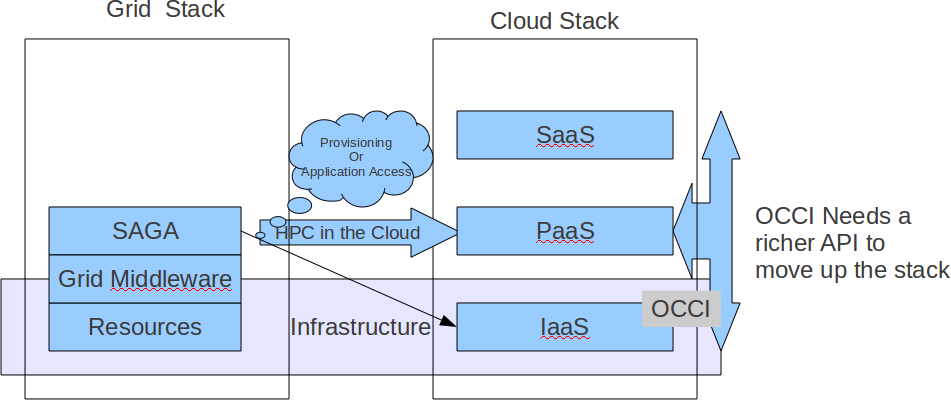
\includegraphics[width=13cm,height=7cm]{figures/prop_position_paper.png}
\caption{Overview of what this paper should demo}
\label{fig:idea}
\end{figure}

\begin{figure}[h]
\centering
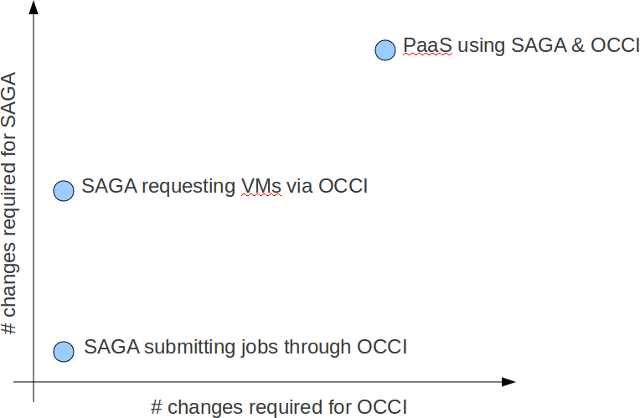
\includegraphics[width=13cm,height=7cm]{figures/changes_on_occi_and_saga.png}
\caption{Changes needed for different models - this picture needs to be refined}
\label{fig:aaS_changes}
\end{figure}

\section{Architecture}

\subsection{3-Level Architecture Diagram}

\bibliographystyle{plain}
\bibliography{inter-cloud-grid-2011}

\end{document}

